% Created 2021-06-11 Fri 16:10
% Intended LaTeX compiler: pdflatex
\documentclass[11pt]{article}
\usepackage[utf8]{inputenc}
\usepackage[T1]{fontenc}
\usepackage{graphicx}
\usepackage{grffile}
\usepackage{longtable}
\usepackage{wrapfig}
\usepackage{rotating}
\usepackage[normalem]{ulem}
\usepackage{amsmath}
\usepackage{textcomp}
\usepackage{amssymb}
\usepackage{capt-of}
\usepackage{hyperref}
\author{Vincent Toups}
\date{\today}
\title{}
\hypersetup{
 pdfauthor={Vincent Toups},
 pdftitle={},
 pdfkeywords={},
 pdfsubject={},
 pdfcreator={Emacs 27.2 (Org mode 9.4.4)}, 
 pdflang={English}}
\begin{document}

\tableofcontents

\section{User Stories For Advanced Asset Browsing}
\label{sec:orgc5f3fa3}

We would like to extend the asset browser to do some meta-data based
search. Implementation details aside, the user stories should be
something like this:

\subsection{User Wants all (Columnar) Data with A Given Column}
\label{sec:orgf075a22}

The user wishes to search for any data set which contains a given
column, for concreteness, say this column is called "QSSCAT".

The asset browser now contains an additional text field hinted with
"query."

\begin{center}
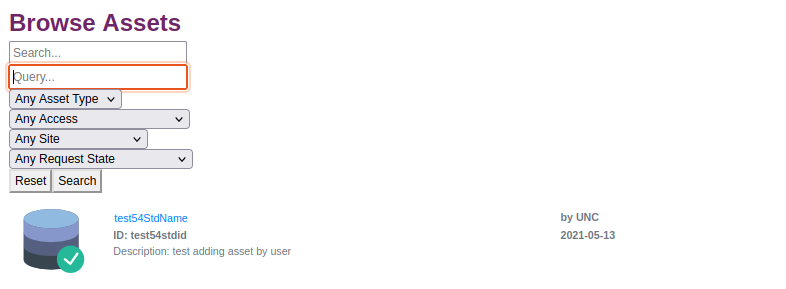
\includegraphics[width=.9\linewidth]{./new-search-box.png}
\end{center}

The user types \texttt{columns :has QSSCAT} and when the search completes any
columnar data with such a column is returned.  In an ideal world the
first and third part of the above query would be auto-completed from a
list of known columns.

\begin{center}
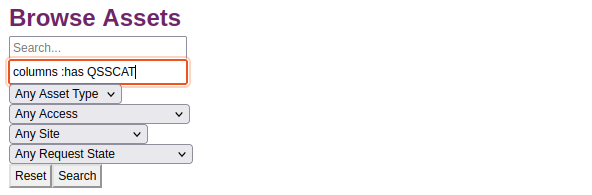
\includegraphics[width=.9\linewidth]{./simple-query.png}
\end{center}

\subsection{User Wants all Columnar Data with a given value in a given column}
\label{sec:orge70e2aa}

In this slightly more complex case the user wishes to find all
columnar data with both a given column and a given value in that
column.

They enter a query like \texttt{columns :has QSSCAT :and QSSCAT :has "PROMIS
Sleep Disturbance"}

\begin{center}
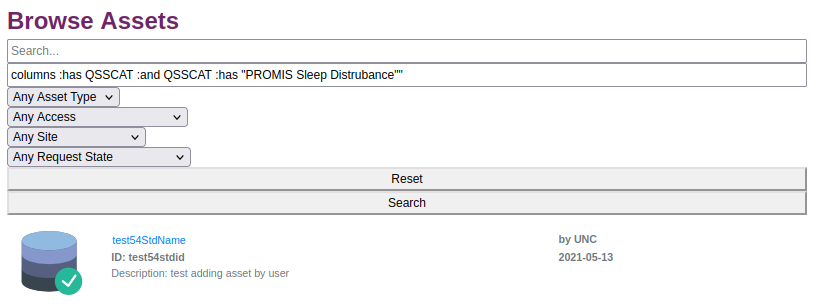
\includegraphics[width=.9\linewidth]{./query2.png}
\end{center}

The result set contains only data sets which have that column and in
which that column contains the value expected.

\subsection{User Wants data with at least one column}
\label{sec:org95fb4a7}

They enter \texttt{columns :has QSSCAT :or \textasciitilde{}columns :has QSSTRESC}

\begin{center}
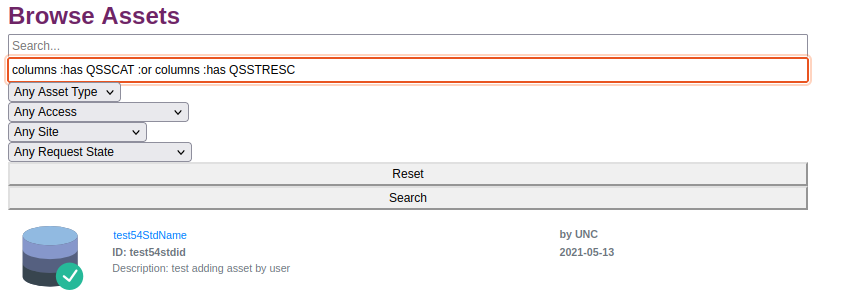
\includegraphics[width=.9\linewidth]{./query3.png}
\end{center}

The results are those data sets with either column.

\subsection{User wants data with at least one column but doesn't want to type as much}
\label{sec:org56c4716}

The user types \texttt{columns :has QSSCAT :or QSSTRESC} which has the same
result as above.

These minimal features are sufficient to form complex queries over the
meta-data data-model described in the "Data Model" document.
\end{document}
